\newpage
\thispagestyle{sectioned}
\chapter{State of the Art}
%\addcontentsline{toc}{chapter}{State of the art}
This chapter will explore the global state of the art related to this work, and the evolution of gadgets and robots along the existence of the Internet.
\section{Generic Overview}
The concept of gadgets might have born with the name of apps in Google's ``Google Personalized Homepage'' in 2005 \cite{ref:what_happened_to_igoogle}, later to be called iGoogle (Figure \ref{fig:igoogle_2008}) and rename these components to gadgets. There is an important distinction to make: Nowadays hearing the words apps reminds us of portable phone applications. The word app insinuates smaller size and lesser complexity, and that is true for both kind of apps, but this work is exploring those \textbf{applications than run inside a bigger environment} and are embedded in it, extending it, but are not standalone and complete by themselves, they depend on the parent framework.
\begin{figure}[h]
  \center
    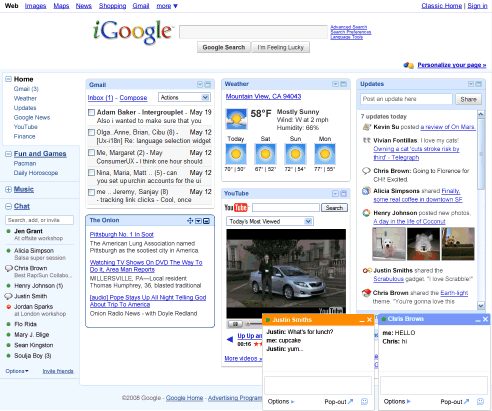
\includegraphics[keepaspectratio, scale=0.6]{Media/Captures/Soa/iGoogle.png}
  \caption{iGoogle in 2008}
  \label{fig:igoogle_2008}
\end{figure}
The social aspect of this apps was being able to share your gadgets with other people, and some examples of them would be weather apps, stock apps or video-watching apps.\\[.2cm]
In the latest years of iGoogle's life, before being discounted in 2012, iGoogle apps coexisted with Google Wave \cite{ref:wave_guide}, and Google Wave's Gadgets (Figure \ref{fig:wave_gadgets}). This other gadgets offered the advantage of the Federated Wave Protocol \cite{ref:wave_federation_protocol} and \textbf{real-time collaboration} \cite{ref:apache_wave_about}.\\[.2cm]
\begin{figure}[h]
  \center
    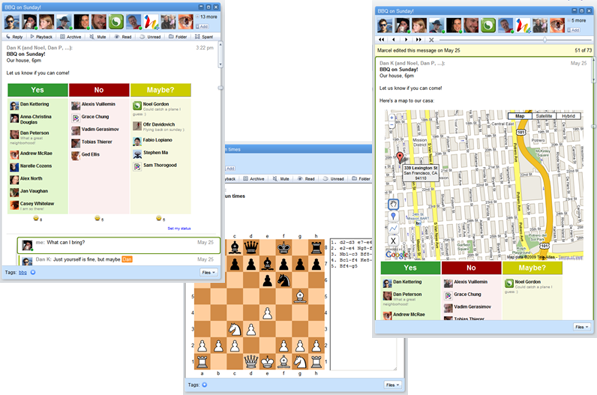
\includegraphics[keepaspectratio, scale=0.5]{Media/Captures/Soa/WaveGadgets.png}
  \caption{Google Wave Gadgets}
  \label{fig:wave_gadgets}
\end{figure}
Then Google began pushing Google+ \cite{ref:google_plus}, which can be considered to have some kind of gadgets in the shape of games, which were heavily influenced by Facebook games \cite{ref:facebook_games}, allowing users to play with other people from the same social networks, giving gifts and sharing scores.\\[.2cm]
Google also briefly had Spreadsheet Gadgets, which added unusual functionality for a spreadsheet application in Google Docs.\\[.2cm]
But Google has not been the only player in the world of applications. In the neat past Flash \cite{ref:adobe_flash} components have been omnipresent, basically for games but not limited for them. Another alternative for applications in the web are Java Applets \cite{ref:java_applets}, commonly use for scientific and learning purposes.\\[.2cm]
The other aspect explored in this work are robots, also known as bots. Robots usually interact loosely coupled from the software they are meant to interact with, but as with Wave Gadgets, robots can be incorporated in the main software, acting as an extension to it. An example of this are uNrEaL Bot \cite{ref:unreal_bot}, a collection of robots for very popular video games created to give the user an advantage over the rest of the players, integrating the graphical interface inside the game, and altering the game's own engine.\\[.2cm]
Robots are also \textbf{important in the web world itself}, but they are not usually productive bots, but instead robots made to emulate human behaviour to trick systems and people and get some kind of profit from it. It has been estimated that one third of the world's Internet traffic is made by automated robots \cite{ref:robots_in_the_web}. But this robots are different in the aspect that they are not meant to be: There is no intended resources for them and they take advantage of vulnerabilities, so as a result they can not run in harmony with the parent software, but as a parasite.

\section{State of the Art for Extensions}
As several extensions will been seen here, the specific state of the art concerning each of them has been explored deeper in their specific chapters \ref{subsec:cc_soa}, \ref{subsec:decision_soa}, \ref{subsec:video_soa} and \ref{subsec:color_soa} respectively, so they are closer to their context.
